\documentclass[border=3pt,tikz]{standalone}
% Shared look for every TikZ figure in these notes.
% Included by each standalone figure file; also keeps the figures consistent
% with the colours used in the PDF and on the website.

\usepackage{tikz}
\usepackage{pgfplots}
\pgfplotsset{compat=1.18}
\usetikzlibrary{arrows.meta, decorations.markings, decorations.pathmorphing,
                patterns, calc, positioning}
\usepackage{amsmath}

% Series colours are the three validated categorical slots also used by the
% interactive widgets, so a path drawn in the printed notes and the same path on
% the website are the same colour. They clear the colour-vision-deficiency and
% contrast checks as a set; every path is direct-labelled as well, so colour is
% never the only thing carrying identity.
\definecolor{duPurple}{HTML}{68246D}
\definecolor{duBlue}{HTML}{2A78D6}
\definecolor{duRed}{HTML}{EB6834}
\definecolor{duGreen}{HTML}{1BAF7A}
\definecolor{duGrey}{HTML}{6B6B6B}

\tikzset{
  axisline/.style   = {-{Stealth[length=3mm]}, line width=0.7pt, black},
  path1/.style      = {duBlue,   line width=1.1pt},
  path2/.style      = {duRed,    line width=1.1pt},
  path3/.style      = {duGreen,  line width=1.1pt},
  statedot/.style   = {circle, fill=black, inner sep=1.4pt},
  arrowhead/.style  = {decoration={markings,
                        mark=at position #1 with {\arrow{Stealth[length=2.6mm]}}},
                       postaction={decorate}},
  lbl/.style        = {font=\small},
  slbl/.style       = {font=\footnotesize, duGrey},
  workfill/.style   = {duPurple, opacity=0.16},
}

% the three simple ideal-gas processes that follow from Pv = RT
\begin{document}
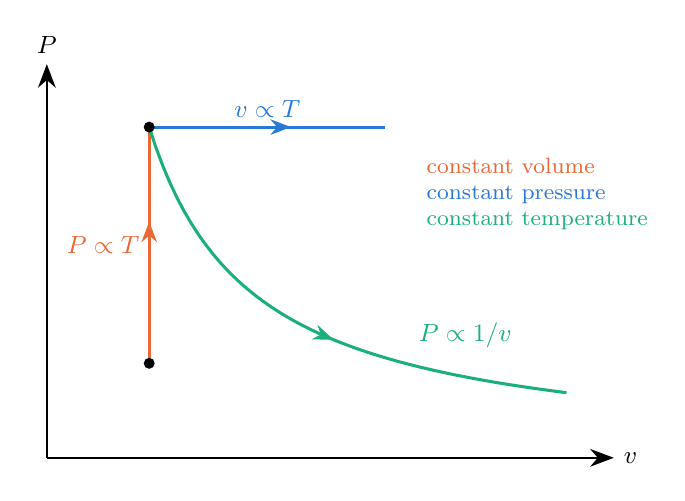
\begin{tikzpicture}[x=1cm,y=1cm]
  \draw[axisline] (0,0) -- (7.2,0) node[right, lbl] {$v$};
  \draw[axisline] (0,0) -- (0,5.0) node[above, lbl] {$P$};
  % constant volume: vertical
  \draw[path2, arrowhead=0.6] (1.3,1.2) -- (1.3,4.2);
  \node[lbl, duRed, left] at (1.3,2.7) {$P \propto T$};
  % constant pressure: horizontal
  \draw[path1, arrowhead=0.6] (1.3,4.2) -- (4.3,4.2);
  \node[lbl, duBlue, above] at (2.8,4.2) {$v \propto T$};
  % constant temperature: hyperbola P = C/v through (1.3,4.2)
  \draw[path3, arrowhead=0.55, domain=1.3:6.6, samples=60] plot (\x, {5.46/\x});
  \node[lbl, duGreen, right] at (4.6,1.55) {$P \propto 1/v$};
  \node[statedot] at (1.3,1.2) {}; \node[statedot] at (1.3,4.2) {};
  % legend
  \node[slbl, anchor=west, align=left] at (4.7,3.35)
    {\textcolor{duRed}{constant volume}\\ \textcolor{duBlue}{constant pressure}\\ \textcolor{duGreen}{constant temperature}};
\end{tikzpicture}
\end{document}
